\documentclass[12pt]{article}
\usepackage{color}
\usepackage{tikz}
\usepackage{amsmath}
\usetikzlibrary{shapes,snakes}

\begin{document}

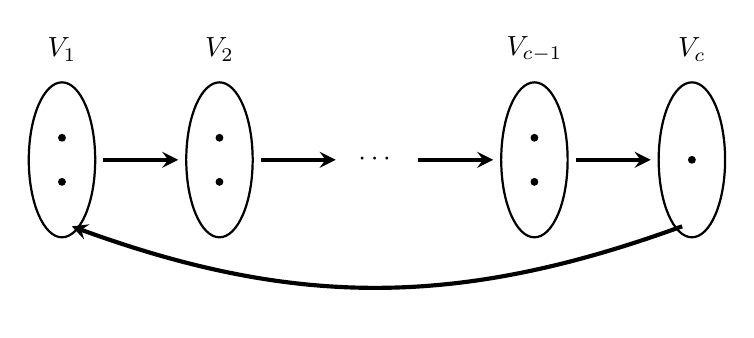
\begin{tikzpicture}[scale=0.4]
	\foreach \i in {(-10,0),(-5,0),(5,0),(10,0)}{\draw[-stealth, line width=0.8pt] \i ellipse [x radius=30pt, y radius=70pt];}
	\coordinate [label=center:$V_1$] () at (-10,3.5);
	\coordinate [label=center:$V_2$] () at (-5,3.5);
	\coordinate [label=center:$\cdots$] () at (0,0);
	\coordinate [label=center:$V_{c-1}$] () at (5,3.5);
	\coordinate [label=center:$V_c$] () at (10,3.5); 
	
	\filldraw[black](-10,0.7) circle (3pt)node[](){};
	\filldraw[black](-10,-0.7) circle (3pt)node[](){};
	\filldraw[black](-5,0.7) circle (3pt)node[](){};
	\filldraw[black](-5,-0.7) circle (3pt)node[](){};
	\filldraw[black](5,0.7) circle (3pt)node[](){};
	\filldraw[black](5,-0.7) circle (3pt)node[](){};
	\filldraw[black](10,0) circle (3pt)node[](){};
	
	
	\filldraw[white](-9,0) circle (0.1pt)node[](u){};
	\filldraw[white](-6,0) circle (0.1pt)node[](v){};
	\filldraw[white](-4,0) circle (0.1pt)node[](u1){};
	\filldraw[white](-1,0) circle (0.1pt)node[](v1){};
	\filldraw[white](1,0) circle (0.1pt)node[](u2){};
	\filldraw[white](4,0) circle (0.1pt)node[](v2){};
	\filldraw[white](6,0) circle (0.1pt)node[](u3){};
	\filldraw[white](9,0) circle (0.1pt)node[](v3){};
	\filldraw[white](10,-2) circle (0.1pt)node[](u4){};
	\filldraw[white](-10,-2) circle (0.1pt)node[](v4){};
	\foreach \i/\j in {u/v,u1/v1,u2/v2,u3/v3}{\draw[-stealth, line width=1.5pt] (\i) edge (\j);}
	\draw[-stealth, line width=1.5pt] (u4) edge[bend left=20] (v4);
	\end{tikzpicture}

\end{document}